\section*{Problem statement}
\addcontentsline{toc}{section}{\protect\numberline{}{Problem statement}}

% alignment types
\begin{figure}[t]  %\begin{floatingfigure}[l]{0.5\textwidth}
    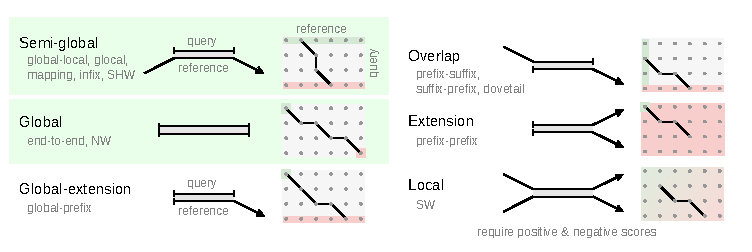
\includegraphics[width=\textwidth]{alignment-types-thesis.pdf}
	\caption[Main alignment types]{Names, alignment, and paths of main alignment
    types. Synonyms of the alignment names are shown in grey. The alignments are
    simplistically shown without edits. Paths corresponding to the alignments
    are shown as paths on an alignment graph. All paths start at green nodes and
    finish at red nodes. With green background are shown the two alignment types
    considered in this thesis.}
    \label{fig:alignment-types}
\end{figure}

\paragraph{Sequence alignment}
One of the simplest operations on sequences is to compare them. We consider the
problem of \emph{pairwise sequence alignment}: given two sequences, we align one
to the other letter-by-letter. Depending on the parts of the sequences that are
being aligned, we distinguish types of alignment~(\cref{fig:alignment-types})
and focus on global and semi-global (shown in green).

There are generalizations to sequence-to-sequence alignment, including aligning
to nonlinear structures, such as directed acyclic graphs, DAGs, and general
graphs. These structures are nowadays becoming more common as a compressed
representation of a set of references to which a sequence can be aligned. One
best alignment is often sufficient, but finding several best (top-K) alignments
is also possible. In the context of read alignment, a set of reads is aligned to
the same reference sequence, so an indexing procedure is often helpful for the
performance.

%If both sequences have to
%be aligned end-to-end, we look for a \emph{global alignment} whose minimal
%number of edits is known as \emph{edit distance}. If we instead search for an
% occurrence of a query sequence within a reference sequence, we allow the
%alignment to start and end at any reference locations in a \emph{semi-global}
%alignment.

\paragraph{Minimizing edits}
Finding alignments would have been relatively easy if the sequences did not
differ. Nevertheless, the real data may be subject to biological evolution and
sequencing technologies, resulting in differences between compared sequences.
Commonly, the most probable explanation of these differences is to be
reconstructed. If we assume an \emph{error model} which repeatedly applies a
random single-letter edit (substitutions, insertions, and deletions), then the
most probable sequence of edits would be one with a minimal number of edits
(possibly weighting different types of edits with different costs). Throughout
this thesis, we consider this most widespread objective---it provides a tradeoff
between expressivity and computability---it reasonably estimates the real-world
sequences while disregarding any memory in the error model.

\paragraph{Global alignment}
The simplest type of alignment is to find a sequence of edits that convert one
whole sequence $A$ to another sequence $B$. Note that converting $A$ to $B$
corresponds to the reverse process of converting $B$ to $A$ (e.g. insertions
correspond to deletions). If we ignore the order of applying the edits, the
result can be equivalently represented simpler as an \emph{alignmnet}: each
letter from $A$ has either not been edited (so it corresponded to a matching
letter in $B$), or has been substituted for another letter (so it corresponded
to a mismatching letter in $B$), or has been deleted (which can be represented
as mismatching it with an inserted fictive \emph{gap symbol} in $B$).
Additionally, letters could have been added to $A$ (represented as a gap in $A$
mismatching a letter in $B$). Note that the number of edits equals the number of
mismatches in the corresponding alignment. The minimal number of edits necessary
to transform $A$ to $B$ is known as \emph{Levenshtein distance} when each edit
operation is equally costly, and more generally as \emph{edit distance} when the
edit operations are weighted depending on their type. Finding an alignment with
a minimal number of edits implies also computing the edit distance.

\paragraph{Semi-global alignment}
Semi-global sequence alignment (also called approximate/fuzzy string search
outside computational biology) is the alignment of a whole \emph{query} sequence
to a continuous region (subsequence) of a \emph{reference} sequence. This region
is unspecified, so semi-global alignment is a more complex problem than global
alignment. We target semi-global alignment by again minimizing edit distance. An
alignment also implies finding a reference region where the query aligns, known
as \emph{mapping} and sufficient for some applications.

\paragraph{Semi-global alignments on the same reference}
If multiple queries have to be aligned on the same reference, powerful
optimizations are applicable.

\paragraph{Sequence-to-graph alignment}
A set of reference sequences can be compactly represented as paths in a graph
(possibly cyclic). \emph{Sequence-to-graph} alignment is a semi-global alignment
between a query sequence and a path in a reference
graph~\cite{jain_complexity_2019}.

\paragraph{Alignment as shortest path}
An alignment of two sequences is a letter-to-letter correspondence between the
two sequences (using gap letters for insertions and deletions). Considering the
corresponding letters consecutively, each pair of letters proceeds to a longer
prefix of $A$ (in case of an insertion), to a longer prefix of $B$ (in case of a
deletion), or to longer prefixes of both (in case of matching or substituted
letters). If we define an \emph{alignment graph} to contain all pairs of
prefixes as nodes and all edits as edges, then any alignment will correspond to
a path. Moreover, if the edges are weighted by the edit costs, any alignment
with a minimal edit distance will correspond to a shortest path. Thus, we will
find the best alignments as shortest paths in an alignment graph.

\paragraph{Objective functions}
Assuming that two sequences align without errors is reasonable only for short
sequences. Otherwise, for sequences of equal length, we can calculate their
\emph{Hamming distance} -- the number of necessary substitution operations to
transform one to the other. Within this thesis, we assume the edit distance and
Levenshtein distance, which also allows for gaps. They can further be
generalized to \emph{affine costs} (starting a gap is more expensive than
extending it), \emph{convex} and \emph{concave} costs (extending the gaps gets
cheaper or more expensive with length), and others. The strive is to balance a
realistic optimization metric and computational efficiency.